\documentclass[11pt,table]{beamer}
\mode<presentation>
\usepackage{etex}
\usepackage{graphicx}
\usepackage{epstopdf}
\usepackage[english]{babel}
\usepackage{tabularx}
\usepackage{booktabs}
\usepackage{mathrsfs}
\usepackage{multicol}
\usepackage{bm}
\usepackage{subcaption}
\usepackage{wrapfig}
\usepackage{dcolumn}
\usepackage{threeparttable}
\usepackage{booktabs}
\usepackage{bbm}
\usepackage{amsmath,dsfont,listings}
\usepackage{amssymb}
\usepackage{rotating}
\usepackage{multirow}
\usepackage{tcolorbox}
\usepackage[authoryear]{natbib}
\usepackage{circledsteps}
\usepackage{qtree}

\usepackage{tikz}
\usetikzlibrary{arrows,decorations.pathmorphing,backgrounds,fit,positioning,shapes.symbols,chains, arrows.meta}
\setbeamertemplate{section in toc}[sections numbered]
\setbeamertemplate{caption}[numbered]

\bibliographystyle{Econometrica}

\setbeamersize{text margin right=3.5mm, text margin left=7.5mm}  % text margin
\setbeamersize{sidebar width left=0cm, sidebar width right=0mm}
\setbeamertemplate{sidebar right}{}
\setbeamertemplate{sidebar left}{}

\definecolor{text-grey}{rgb}{0.45, 0.45, 0.45} % grey text on white background
\definecolor{bg-grey}{rgb}{0.66, 0.65, 0.60} % grey background (for white text)
\definecolor{fu-blue}{RGB}{0, 51, 102} % blue text
\definecolor{fu-green}{RGB}{153, 204, 0} % green text
\definecolor{fu-red}{RGB}{204, 0, 0} % red text (used by \alert)
\definecolor{BrewerBlue}{HTML}{377EB8} % Define Brewer Blue
\definecolor{BrewerRed}{HTML}{E41A1C}  % Define Brewer Red
\definecolor{lightblue}{rgb}{0.8,0.85,1}

\setbeamertemplate{frametitle}{%
    \vskip-30pt \color{text-grey}\large%
    \begin{minipage}[b][23pt]{\textwidth}%
    \flushleft\insertframetitle%
    \end{minipage}%
}

\setbeamertemplate{navigation symbols}{} 

%%% begin title page
\setbeamertemplate{title page}{
\vskip2pt\hfill
\vskip19pt\hskip3pt

% set the title and the author
\vskip4pt
\parbox[top][1.35cm][c]{11cm}{\LARGE\color{text-grey} \textcolor{red1}{RL}earning:\\[1ex] \inserttitle \\[1ex] \small \quad \\[3ex]}
\vskip17pt
\parbox[top][1.35cm][c]{11cm}{\small Unit 1-1: \insertsubtitle \\[2ex] \insertauthor \\[1ex]}
}
%%% end title page

%%% colors
\usecolortheme{lily}
\setbeamercolor*{normal text}{fg=black,bg=white}
\setbeamercolor*{alerted text}{fg=fu-red}
\setbeamercolor*{example text}{fg=fu-green}
\setbeamercolor*{structure}{fg=fu-blue}

\setbeamercolor*{block title}{fg=white,bg=black!50}
\setbeamercolor*{block title alerted}{fg=white,bg=black!50}
\setbeamercolor*{block title example}{fg=white,bg=black!50}

\setbeamercolor*{block body}{bg=black!10}
\setbeamercolor*{block body alerted}{bg=black!10}
\setbeamercolor*{block body example}{bg=black!10}

\setbeamercolor{bibliography entry author}{fg=fu-blue}
\setbeamercolor{bibliography entry journal}{fg=text-grey}
\setbeamercolor{item}{fg=fu-blue}
\setbeamercolor{navigation symbols}{fg=text-grey,bg=bg-grey}
%%% end colors

%%% headline
\setbeamertemplate{headline}{
\vskip30pt
}
%%% end headline

%%% footline
\newcommand{\footlinetext}{
%\insertshortinstitute, \insertshorttitle, \insertshortdate
}
\setbeamertemplate{footline}{
\vskip2pt
\hfill \raisebox{-1pt}{\usebeamertemplate***{navigation symbols}}
\hfill \insertframenumber\hspace{10pt}
\vskip4pt
}
%%% end footline

%%% settings for listings package
\lstset{extendedchars=true, showstringspaces=false, basicstyle=\footnotesize\sffamily, tabsize=2, breaklines=true, breakindent=10pt, frame=l, columns=fullflexible}
\lstset{language=Java} % this sets the syntax highlighting
\lstset{mathescape=true} % this switches on $...$ substitution in code
% enables UTF-8 in source code:
\lstset{literate={ä}{{\"a}}1 {ö}{{\"o}}1 {ü}{{\"u}}1 {Ä}{{\"A}}1 {Ö}{{\"O}}1 {Ü}{{\"U}}1 {ß}{\ss}1}
%%% end listings

\usepackage{concmath}
\usepackage{xcolor}
\definecolor{red1}{RGB}{206, 17, 38}
\definecolor{blue1}{RGB}{16, 118, 208}
\definecolor{gray1}{RGB}{117, 115, 115}
\usepackage{hyperref}


\newtheorem{proposition}{Proposition}
\newtheorem{assumption}{Definition}

\title[]{Short guides to reinforcement learning}
\subtitle[]{Multi-Armed Bandits}
\author[D. Rostam-Afschar]{\textcolor{gray1}{Davud Rostam-Afschar (Uni Mannheim)}}
\date[]{\today}
\subject{Econometrics}
\renewcommand{\footlinetext}{\insertshortinstitute, \insertshorttitle, \insertshortdate}
\hypersetup{
    bookmarks=false,
    unicode=false,
    pdftoolbar=false,
    pdffitwindow=true,
    pdftitle={Reinforcement Learning for Business, Economics, and Social Sciences: \insertsubtitle},
    pdfauthor={Davud Rostam-Afschar},
    pdfsubject={Reinforcement Learning},
    pdfkeywords={reinforcement learning, Multi-Armed Bandits},
    pdfnewwindow=true,
}
\def\sym#1{\ifmmode^{#1}\else\(^{#1}\)\fi}

\begin{document}

\begin{frame}[plain]
  \titlepage
\end{frame}

% --------------------------------------------------- Slide --
%\begin{frame}
	%\frametitle{Content}
	%\tableofcontents[]
%\end{frame}



\section{Multi-Armed Bandits}


{
\setbeamercolor{background canvas}{bg=BrewerBlue}
\begin{frame}
\centering
\Huge
\textcolor{white}{How to assign treatments adaptively?}
\thispagestyle{empty}
\end{frame}
}



\renewcommand{\baselinestretch}{1}




\begin{frame}\frametitle{Adaptive Experimental Designs}
\renewcommand{\baselinestretch}{1}
\begin{itemize}
    \item Randomized controlled trials gold standard of causal inference
    \item Adaptive experiments allow ``earning while learning''
    \item Push to replace non-adaptive randomized trials with bandits\pause
    \begin{itemize}
        \item In medicine, economics, political science, survey methods research, education, psychology, \ldots
        \item Practitioners use bandit algorithms\pause
        \item Can improve outcomes for participants (optimize regret)
        \item Can improve policies learned at the end of trial (best-arm identification)\pause
    \end{itemize}
    \item Some popular algorithms\pause
    \begin{itemize}
        \item $\varepsilon$-first\pause
        \item $\varepsilon$-greedy\pause
        \item Upper Confidence Bound\pause
        \item Thompson sampling
    \end{itemize}
\end{itemize}

\end{frame}


\begin{frame}\frametitle{Stylized Data Structure}
\renewcommand{\baselinestretch}{1}
\begin{figure}[h]
\begin{center}
{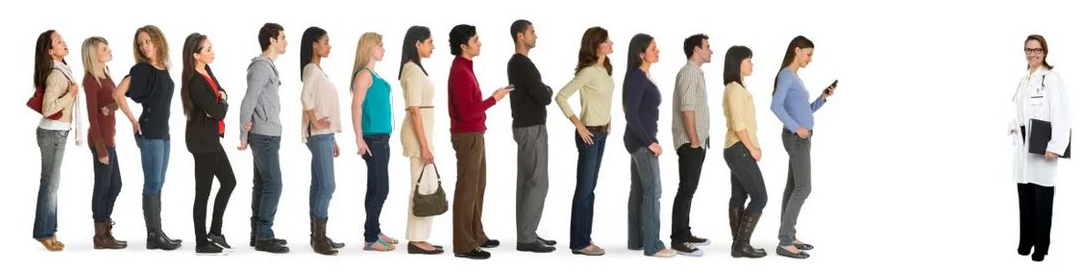
\includegraphics[width=0.9\textwidth]{figures/queue.png}}
\end{center}
\end{figure}
\begin{columns} 

    \begin{column}{.55\textwidth}       \vspace{-2ex}

\begin{table}[htbp]

\label{tab:data_structure}
\begin{threeparttable}
\tiny
\begin{tabular}{@{\extracolsep{-5pt}}l*{3}{c}}
\toprule
Obs & Selected Arm & Reward\\
\midrule
1 & A & 0  \\
2 & B & 0 \\
3 & A & 1 \\
4 & B & 0 \\
5 & A & 0 \\
6 & B & 1 \\
7 & A & 1 \\
8 & B & 0 \\
9 & A & 0 \\
10 & A & 1\\
11 & A & 1\\
12 & B & 0\\
13 & A & 1\\
14 & A & 0\\
15 & A & 1\\
16 & B & 0\\

\bottomrule
\end{tabular}

\end{threeparttable}
\end{table}

\renewcommand{\baselinestretch}{1.45}
    \end{column}%
     \begin{column}{.5\textwidth}       \vspace{-2ex}

\begin{itemize}
    \item Does arm A or arm B\\ perform better?\\[2ex]
    \item Which arm to play\\ in next trial (round 17)?
\end{itemize}
\end{column}
\end{columns}

\end{frame}




\begin{frame}{Multi-Armed Bandits as a Reinforcement Learning Problem}

    \begin{center}

\begin{tikzpicture}[node distance=1cm]
\node[fill=lightgray!40!white,rectangle,draw,rounded corners=2pt,inner sep=1ex,line width=1.5pt,minimum height=0.8cm] (O) {\large Bandit Algorithm};
\node[draw,fill=lightgray!40!white,line width=1.5pt, rectangle,rounded corners=2pt,minimum height=1cm,below=of O] (A) {Environment};

%left Path connect
%\draw[line width=1.2pt,latex-]  ([yshift=2mm]O.west) -- ++(-3,0) |- ([yshift=-2mm]A.west) node[pos=0.25,left,align=right,font=\scriptsize] { state\\ $S_t$};
\draw[line width=0.7pt,latex-]  ([yshift=-0.5mm]O.west) -- ++(-2.5,0) |- ([yshift=2.5mm]A.west) node[pos=0.25,right,align=left,font=\scriptsize] { reward=-regret\\ $R_t$};

%right Path connect
\draw[line width=1.2pt,-latex]  (O.east) -- ++(2.0,0) |- (A.east) node[pos=0.25,right,align=left,font=\scriptsize] {select arm\\ $A_t$};

%\draw[-{Latex[scale=1.5]}] ([yshift=-2mm]A.west) -- ++(-1,0) node[pos=0.4,above=-1pt,font=\scriptsize] {$S_{t+1}$};
\draw[-{Latex[scale=1.2]}] ([yshift=2.5mm]A.west) -- ++(-1,0) node[pos=0.4,above=-1pt,font=\scriptsize] {$R_{t+1}$};


\draw[yshift=-1.9cm,xshift=-2.11cm,line width=1pt,densely dashed] (0,-0.5)--(0,0.5) node[below,pos=0,font=\scriptsize] {next step};
\end{tikzpicture}\\
\vspace{3mm}
  {Goal:} Learn to choose actions that maximize rewards

\end{center}
    
\end{frame}

\begin{frame}{What Are Multi-Armed Bandits?}
    \begin{columns}
        \begin{column}{0.65\textwidth}
            \begin{itemize}
                \item A sequential decision-making problem
                \item Agent chooses among $K$ options (``arms'') repeatedly
                \item Each arm gives an unknown reward
                \item Objective: Maximize total reward\\ (or minimize \textbf{regret})
                \item Core tradeoff:\\ Learning vs. Earning
            \end{itemize}
        \end{column}
        \begin{column}{0.35\textwidth}
            \centering
            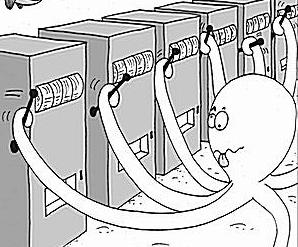
\includegraphics[width=\textwidth]{figures/microsoft research.jpg}
            
            \vspace{0.2em}
            {\scriptsize Microsoft Research}
        \end{column}
    \end{columns}
		\vspace{2ex}
 \pause But how to balance \textbf{exploration} and \textbf{exploitation}?
\end{frame}


\section{Bandit Algorithms}
{
\setbeamercolor{background canvas}{bg=BrewerBlue}
\begin{frame}
\centering
\Huge
\textcolor{white}{Bandit Algorithms}
\thispagestyle{empty}
\end{frame}
}



\begin{frame}{The Exploration/Exploitation Dilemma}
\begin{itemize}
  \item The action-value is the true but unknown mean reward for action $a$:
  \[
  q(a) = \mathbb{E}[R_t \mid A_t = a], \quad \forall a \in \{1, \dots, k\}
  \]
  \item Estimate expected return:
  \[
  Q_t(a) \approx q(a), \quad \forall a \text{ (action-value estimates)}
  \]
  \item Define the greedy action at time $t$ as:
  \[
  A_t^* = \arg\max_a Q_t(a)
  \]
  \item If $A_t = A_t^*$ then you are \textbf{exploiting}
  \item If $A_t \neq A_t^*$ then you are \textbf{exploring}
\end{itemize}
\end{frame}

\begin{frame}{Regret}
\begin{itemize}
  \item The optimal value is:
  \[
  r^* = q(a^*) = \max_{a \in \mathcal{A}} q(a)
  \]
  \item The regret is the opportunity loss for one step:
  \[
  \text{loss}_t = \mathbb{E}[r^* - q(a_t)]
  \]
  \item The total regret is the total opportunity loss:
  \[
  \text{Loss}_T = \sum_{t=1}^{T}\text{loss}_t = \mathbb{E}\left[ \sum_{t=1}^{T} r^* - q(a_t) \right]
  \]

\end{itemize}
\end{frame}






\begin{frame}\frametitle{Stylized Data Structure: Per-Arm = Per-Round Regrets}
\renewcommand{\baselinestretch}{1}
\begin{figure}[h]
\begin{center}
{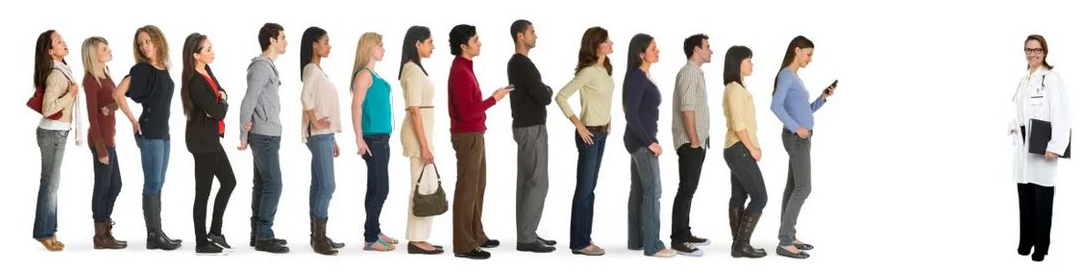
\includegraphics[width=0.9\textwidth]{figures/queue.png}}
\end{center}
\end{figure}
\begin{columns} 

    \begin{column}{.4\textwidth}       \vspace{-2ex}

\begin{table}[htbp]

\label{tab:data_structure}
\begin{threeparttable}
\tiny
\begin{tabular}{@{\extracolsep{-5pt}}l*{3}{c}}
\toprule
Obs $t$ & Selected Arm $a_t$ & Reward $r_t$\\
\midrule
1 & A & \only<1,3->{0}\only<2>{\textcolor{red1}0}  \\
2 & B & \only<1-2,4->{0}\only<3>{\textcolor{red1}0} \\
3 & A & \only<1,3->{1}\only<2>{\cellcolor{lightblue}\textcolor{red1}1} \\
4 & B & \only<1-2,4->{0}\only<3>{\textcolor{red1}0} \\
5 & A & \only<1,3->{0}\only<2>{\textcolor{red1}0} \\
6 & B & \only<1-2,4->{1}\only<3>{\cellcolor{lightblue}\textcolor{red1}1} \\
7 & A & \only<1,3->{1}\only<2>{\cellcolor{lightblue}\textcolor{red1}1} \\
8 & B & \only<1-2,4->{0}\only<3>{\textcolor{red1}0} \\
9 & A & \only<1,3->{0}\only<2>{\textcolor{red1}0} \\
10 & A & \only<1,3->{1}\only<2>{\cellcolor{lightblue}\textcolor{red1}1}\\
11 & A & \only<1,3->{1}\only<2>{\cellcolor{lightblue}\textcolor{red1}1}\\
12 & B & \only<1-2,4->{0}\only<3>{\textcolor{red1}0}\\
13 & A & \only<1,3->{1}\only<2>{\cellcolor{lightblue}\textcolor{red1}1}\\
14 & A & \only<1,3->{0}\only<2>{\textcolor{red1}0}\\
15 & A & \only<1,3->{1}\only<2>{\cellcolor{lightblue}\textcolor{red1}1}\\
16 & B & \only<1-2,4->{0}\only<3>{\textcolor{red1}0}\\

\bottomrule
\end{tabular}

\end{threeparttable}
\end{table}

\renewcommand{\baselinestretch}{1.2}
    \end{column}%
     \begin{column}{.6\textwidth}       \vspace{-2ex}
\begin{enumerate}\scriptsize
\only<2-4>{
  \item[1.] \textbf{Compute counts \& empirical means}
  \begin{itemize}\scriptsize

    \item Total pulls: $T=16$
    \item Arm A: $N_{16}(A)=\only<3->{10}\only<2>{\textcolor{red1}{10}}$, $\sum_{t:a_t=A}r_t=\only<3->{6}\only<2>{\textcolor{red1}{6}}$\\[2ex] $\implies q(A)=6/10=0.6$\\[4ex]
    \uncover<3-4>{\item Arm B: $N_{16}(B)=\only<2,4->{6}\only<3>{\textcolor{red1}{6}}$,  $\sum_{t:a_t=B}r_t=\only<2,4->{1}\only<3>{\textcolor{red1}{1}}$\\[2ex] $\implies q(B)=1/6\approx0.1667$}
  \end{itemize}
}
\uncover<4>{
  \item[2.] \textbf{Identify the optimal arm and its mean}
  \[ r^* = \max\{q(A),q(B)\} = 0.6 \]
}
\only<5-8>{\vspace{-2cm}
  \item[3.] \textbf{Sum of per-round regrets}\vspace{-0.25cm}
  \uncover<5-8>{  \[
    \text{Loss}_{16}=\sum_{t=1}^{16}(r^*-q(a_t))
  \]}\vspace{-0.35cm}
	\uncover<6-8>{
  \begin{itemize}\scriptsize

    \item For $a_t=A$: $r^*-q(A)=0.6-0.6=0$
    \uncover<7-8>{\item For $a_t=B$: $r^*-q(B)=0.6-0.1667\approx0.4333$\\[2ex]}
		\uncover<8>{
		Played 6 times:
    \[
      \text{Loss}_{16}=6\times0.4333\approx2.6
    \]
		}
  \end{itemize}
}}
\only<9>{\vspace{-4.4cm}
  \item[4.] \textbf{Sum of per-arm regrets}
  \[
    \sum_{a\in\{A,B\}}N_{16}(a)(r^*-q(a))
  \]
  \[
    =10\times0 + 6\times0.4333 \approx2.6
  \]  
}
\end{enumerate}


\end{column}
\end{columns}

\end{frame}




\begin{frame}{Regret Decomposition Lemma}
\begin{itemize}
  \item Number of times action $a$ has been selected prior to time $t$ $N_t(a)=\sum_{i=1}^{t-1} \mathds{1} \{A_i = a\}$ 
  \item Total regret can be rewritten as:
  \[
  \text{Loss}_t = \mathbb{E}\left[ \sum_{t=1}^{T} r^* - q(a_t) \right] 
  \]
  \[
  = \sum_{a \in \mathcal{A}} \mathbb{E}[N_t(a)]  (r^* - q(a)) 
  \]
\end{itemize}
\begin{itemize}
	\item Regret comes from pulling suboptimal arms
	\item Each arm $a$ contributes $(r^* - q(a))$ for every time $N_t(a)$ it's chosen
\end{itemize}
\end{frame}



\begin{frame}\frametitle{Stylized Data Structure}
\renewcommand{\baselinestretch}{1}
\begin{figure}[h]
\begin{center}
{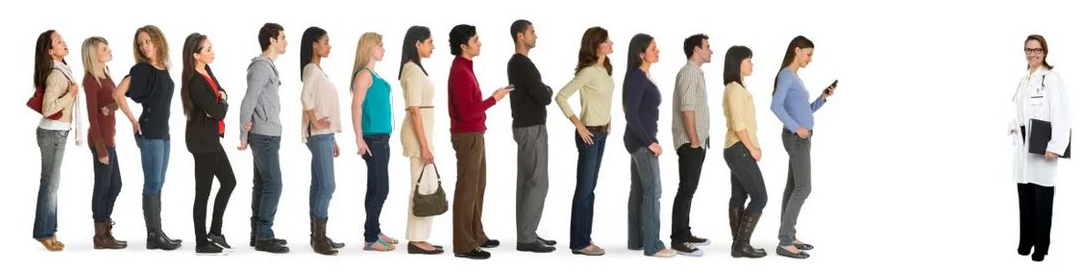
\includegraphics[width=0.9\textwidth]{figures/queue.png}}
\end{center}
\end{figure}


\begin{table}[htbp]

\label{tab:data_structure}
\begin{threeparttable}
\tiny
\begin{tabular}{@{\extracolsep{-5pt}}l*{7}{c}}
\toprule
   $t$ 
   & Arm 
   & Reward 
   & \uncover<3->{$\sum_{i=1}^{n} R_i$} 
   & \uncover<4->{$n$} 
   & \uncover<5->{$Q_n$} 
   & \uncover<6->{$Q_{n-1}$} \\
\midrule
 1  & A & \only<1>{0}\only<2->{\cellcolor{lightblue}0} & \uncover<3->{0} & \uncover<4->{1}  & \uncover<5->{0.00} & \uncover<6->{0.00}  \\
 2  & B & 0 &           \\
 3  & A & \only<1>{1}\only<2->{\cellcolor{lightblue}1} & \uncover<3->{1} & \uncover<4->{2}  & \uncover<5->{0.50} & \uncover<6->{0.00}  \\  
 4  & B & 0 &           \\
 5  & A & \only<1>{0}\only<2->{\cellcolor{lightblue}0} & \uncover<3->{1} & \uncover<4->{3}  & \uncover<5->{0.33} & \uncover<6->{0.50}  \\   
 6  & B & 1 &           \\      
 7  & A & \only<1>{1}\only<2->{\cellcolor{lightblue}1} & \uncover<3->{2} & \uncover<4->{4}  & \uncover<5->{0.50} & \uncover<6->{0.33} \\  
 8  & B & 0 &            \\      
 9  & A & \only<1>{0}\only<2->{\cellcolor{lightblue}0} & \uncover<3->{2} & \uncover<4->{5}  & \uncover<5->{0.40} & \uncover<6->{0.50}  \\  
10  & A & \only<1>{1}\only<2->{\cellcolor{lightblue}1} & \uncover<3->{3} & \uncover<4->{6}  & \uncover<5->{0.50} & \uncover<6->{0.40}  \\  
11  & A & \only<1>{1}\only<2->{\cellcolor{lightblue}1} & \uncover<3->{4} & \uncover<4->{7}  & \uncover<5->{0.57} & \uncover<6->{0.50}  \\   
12  & B & 0 &             \\     
13  & A & \only<1>{1}\only<2->{\cellcolor{lightblue}1} & \uncover<3->{5} & \uncover<4->{8}  & \uncover<5->{0.63} & \uncover<6->{0.57}  \\   
14  & A & \only<1>{0}\only<2->{\cellcolor{lightblue}0} & \uncover<3->{5} & \uncover<4->{9}  & \uncover<5->{0.56} & \uncover<6->{0.63}  \\  
15  & A & \only<1>{1}\only<2->{\cellcolor{lightblue}1} & \uncover<3->{6} & \uncover<4->{10} & \uncover<5->{0.60} & \uncover<6->{0.56}  \\
16  & B & 0 &                          \\
\bottomrule
\end{tabular}
\end{threeparttable}


\end{table}



\end{frame}





\begin{frame}{Incremental Update}
\renewcommand{\baselinestretch}{0.8}
\begin{itemize}
  \item Let $R_1, \dots, R_n$ be rewards received after selecting an action $n$ times.
  \item Define $Q_n$ as the estimate after $n-1$ rewards:
\end{itemize}

\[
Q_n = \frac{1}{n-1} \sum_{i=1}^{n-1} R_i
\]

\begin{itemize}
  \item Now, after receiving the $n$-th reward $R_n$, we update:
\end{itemize}

\[
Q_{n+1} = \frac{1}{n} \sum_{i=1}^{n} R_i = \frac{1}{n} \left( R_n + \sum_{i=1}^{n-1} R_i \right)
\]

\[
= \frac{1}{n} \left( R_n + (n-1) Q_n \right) = Q_n + \frac{1}{n} \left( R_n - Q_n \right)
\]

\pause
\begin{itemize}
  \item This is the incremental update rule:\\
$\underbrace{Q_{n+1}}_{\uncover<2->{\text{\textcolor{red1}{New}}}} = 
\underbrace{Q_n}_{\uncover<2->{\text{\textcolor{red1}{Old}}}} + 
\underbrace{\frac{1}{n}}_{\uncover<2->{\text{\textcolor{red1}{Step size}}}} 
\underbrace{(R_n - Q_n)}_{\uncover<2->{\text{\textcolor{red1}{Error}}}}
$
\end{itemize}
\pause We can get a new estimate without storing all the rewards.

\end{frame}


\begin{frame}\frametitle{Stylized Data Structure: Learning Expected Return}
\renewcommand{\baselinestretch}{1}
\begin{figure}[h]
\begin{center}
{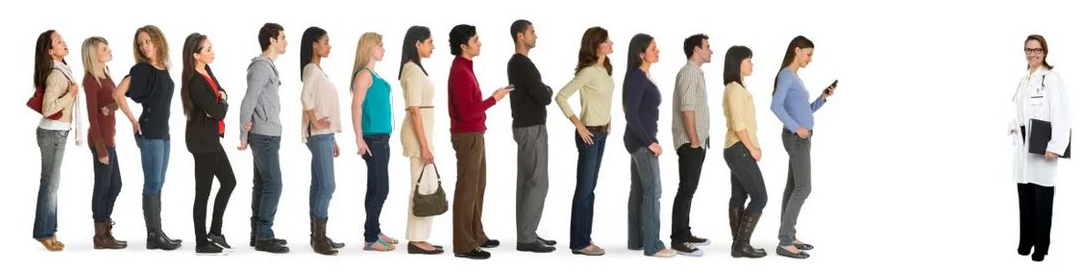
\includegraphics[width=0.9\textwidth]{figures/queue.png}}
\end{center}
\end{figure}


\begin{table}[htbp]

\label{tab:data_structure}
\begin{threeparttable}
\tiny
\begin{tabular}{@{\extracolsep{-5pt}}l*{8}{c}}
\toprule
   $t$ 
   & Arm 
   & Reward 
   & \uncover<3->{$Q_{n-1}$} 
   & \uncover<4->{Update}
   & \uncover<5->{$Q_n$} \\
\midrule
 1  & A & \only<1>{0}\only<2->{\cellcolor{lightblue}0} & \uncover<3->{0.00} & \uncover<4->{%
      $0.00 + \tfrac{1}{1}(0 - 0.00)$} & \uncover<5->{0.00} \\
 2  & B & 0 &           \\
 3  & A & \only<1>{1}\only<2->{\cellcolor{lightblue}1} & \uncover<3->{0.00} & \uncover<4->{%
      $0.00 + \tfrac{1}{2}(1 - 0.00)$} & \uncover<5->{0.50}\\  
 4  & B & 0 &           \\
 5  & A & \only<1>{0}\only<2->{\cellcolor{lightblue}0} & \uncover<3->{0.50} & \uncover<4->{%
      $0.50 + \tfrac{1}{3}(0 - 0.50)$}  & \uncover<5->{0.33}\\   
 6  & B & 1 &           \\      
 7  & A & \only<1>{1}\only<2->{\cellcolor{lightblue}1} & \uncover<3->{0.33} & \uncover<4->{%
      $0.33 + \tfrac{1}{4}(1 - 0.33)$} & \uncover<5->{0.50}\\  
 8  & B & 0 &            \\      
 9  & A & \only<1>{0}\only<2->{\cellcolor{lightblue}0} &  \uncover<3->{0.50} & \uncover<4->{%
      $0.50 + \tfrac{1}{5}(0 - 0.50)$} & \uncover<5->{0.40}\\  
10  & A & \only<1>{1}\only<2->{\cellcolor{lightblue}1} & \uncover<3->{0.40} & \uncover<4->{%
      $0.40 + \tfrac{1}{6}(1 - 0.40)$}  & \uncover<5->{0.50} \\  
11  & A & \only<1>{1}\only<2->{\cellcolor{lightblue}1} & \uncover<3->{0.50} & \uncover<4->{%
      $0.50 + \tfrac{1}{7}(1 - 0.50)$} & \uncover<5->{0.57}\\   
12  & B & 0 &             \\     
13  & A & \only<1>{1}\only<2->{\cellcolor{lightblue}1} & \uncover<3->{0.57} & \uncover<4->{%
      $0.57 + \tfrac{1}{8}(1 - 0.57)$}  & \uncover<5->{0.63}\\   
14  & A & \only<1>{0}\only<2->{\cellcolor{lightblue}0} &  \uncover<3->{0.63} & \uncover<4->{%
      $0.63 + \tfrac{1}{9}(0 - 0.63)$}  & \uncover<5->{0.56}\\  
15  & A & \only<1>{1}\only<2->{\cellcolor{lightblue}1} & \uncover<3->{0.56} & \uncover<4->{%
      $0.56 + \tfrac{1}{10}(1 - 0.56)$} & \uncover<5->{0.60}\\
16  & B & 0 &                          \\
\bottomrule
\end{tabular}
\end{threeparttable}


\end{table}

\end{frame}



\begin{frame}{Sublinear Regret}
Most multi-armed bandit (MAB) algorithms aim to achieve sublinear regret, so that the \textit{average} regret vanishes as the number of rounds $T \to \infty$:

\[
\lim_{T \to \infty} \frac{\text{Loss}_T}{T} = 0
\]

\vspace{1em}
\begin{figure}
	\centering
		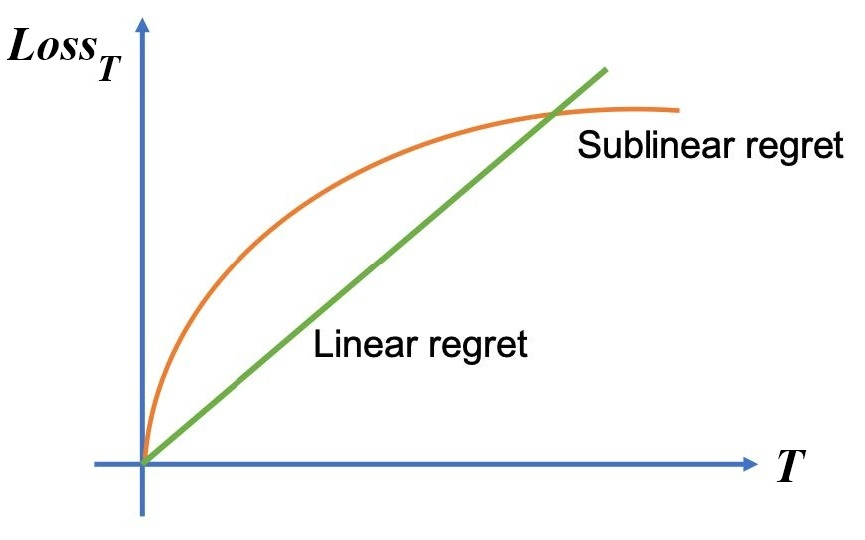
\includegraphics[width=0.50\textwidth]{figures/sublinear regret.jpg}
	\label{fig:sublinear regret}
\end{figure}

\begin{itemize}
    \item $\text{Loss}_T$: expected total expected regret after $T$ rounds.
\end{itemize}  
	
\end{frame}


\begin{frame}{Exploration Strategies for Stochastic Bandits}

\renewcommand{\arraystretch}{1.6}
\footnotesize
\begin{table}[H]
\centering
%\resizebox{\textwidth}{!}{%
\begin{tabular}{ll}
\toprule
\textbf{Algorithm} &  \textbf{Total Regret}  \\
\midrule
\textit{greedy} &
$\mathcal{O}(T)$ \pause\\

\textit{$\varepsilon$-first} &
$\mathcal{O}(T)$  \pause\\

\textit{$\varepsilon$-greedy} &
$\mathcal{O}(T)$  \pause\\

\textit{$\varepsilon$-greedy (decaying)} &
$\mathcal{O}(\log T)$  \pause\\

\textit{UCB (Upper Confidence Bound)} &
$\mathcal{O}(\log T)$  \pause\\

\textit{Thompson Sampling} &
$\mathcal{O}(\log T)$  \pause\\
\bottomrule
\end{tabular}%
%}
\end{table}
\uncover<7->{ Overviews: \cite{Slivkins2019}, \cite{Burtini2015}, \cite{Bubeck2012}}
\end{frame}

\section{Bandits in Practice}
{
\setbeamercolor{background canvas}{bg=BrewerBlue}
\begin{frame}
\centering
\Huge
\textcolor{white}{Bandits in Practice}
\thispagestyle{empty}
\end{frame}
}

\begin{frame}{Real World Bandit: \textit{Netflix Artwork}}
\small
    \begin{itemize}
        \item For a particular movie, which image to show to users on Netflix?
        \item \textbf{Actions:} Choose one of \( k \) images to display
        \item \textbf{Ground-truth mean rewards (unknown):}\\ True percentage of users who click on image and watch movie
        \item \textbf{Estimated mean rewards:}\\ Average observed click-through rates for each image
    \end{itemize}
    \vspace{1em}
    \begin{center}
        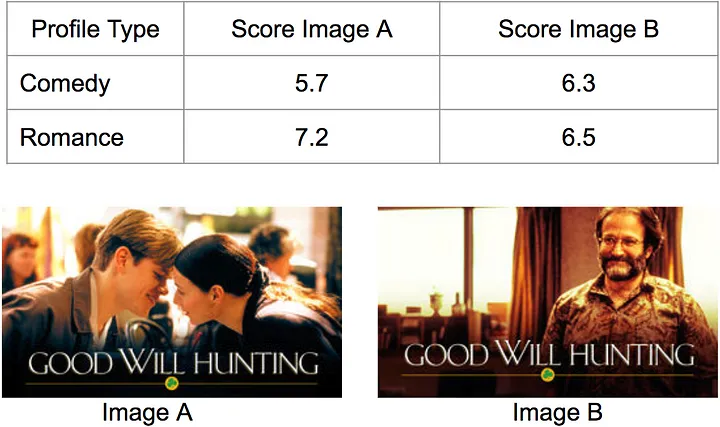
\includegraphics[width=0.45\linewidth]{figures/good will hunting contextual}
        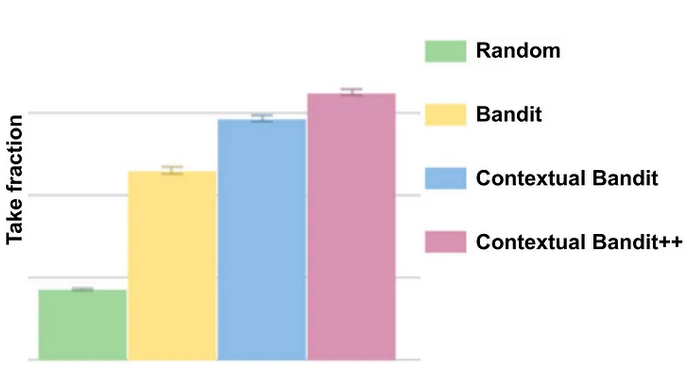
\includegraphics[width=0.45\linewidth]{figures/take fraction}
				
    \end{center}
    \vspace{0.5em}
    \small{Source: \href{https://medium.com/netflix-techblog/artwork-personalization-c589f074ad76}{Netflix Tech Blog}}
\end{frame}


\begin{frame}[t,allowframebreaks
]%\nocite{*}
\frametitle{References}
\small
\bibliography{bib}
\end{frame}



\section{Takeaways}
{
\setbeamercolor{background canvas}{bg=BrewerBlue}
\begin{frame}
\centering
\Huge
\textcolor{white}{Takeaways}
\thispagestyle{empty}
\end{frame}
}

\begin{frame}{How to Balance Earning and Learning?}
\begin{itemize}
    \item Multi-Armed Bandits (MAB) model adaptive, sequential decision-making under uncertainty
    \item Core trade-off: Exploration vs.\ Exploitation
    \item Objective: Maximize total reward, or equivalently, minimize regret
    \item Key algorithms:
    \begin{itemize}
        \item \(\varepsilon\)-first, \(\varepsilon\)-greedy (fixed or decaying)
        \item UCB (Upper Confidence Bound)
        \item Thompson Sampling (Bayesian approach)
    \end{itemize}
\end{itemize}
\end{frame}


\appendix
{
\setbeamercolor{background canvas}{bg=BrewerBlue}
\begin{frame}
\centering
\Huge
\textcolor{white}{Appendix}
\thispagestyle{empty}
\end{frame}
}


\begin{frame}{Regret Decomposition Lemma}
\begin{itemize}
\item Sample mean reward $\mathbb{E}[q(a_t)]$ is true mean reward $q(a)$ times average number of times actions $a$ was chosen
$$\mathbb{E}[q(a_t)]=\mathbb{E}\bigg[\sum_{a \in \mathcal{A}} q(a)\mathds{1} \{A_i = a\}\bigg]=\sum_{a \in \mathcal{A}} q(a)\mathbb{E}[\mathds{1} \{A_i = a\}]$$\\\pause
  \item Total regret can be rewritten as:
  \[
  \text{Loss}_t = \sum_{i=1}^{t-1}\mathbb{E}[r^* - q(a_t)]  \]\pause 
 \[= \sum_{i=1}^{t-1}\left[\sum_{a \in \mathcal{A}} r^*\mathbb{E}[\mathds{1} \{A_i = a\}] - \sum_{a \in \mathcal{A}} q(a)\mathbb{E}[\mathds{1} \{A_i = a\}]\right]
  \]\pause 
 \[
  = \sum_{i=1}^{t-1}\sum_{a \in \mathcal{A}}\mathbb{E}\left[\mathds{1} \{A_i = a\}\right](r^* -  q(a)) = \sum_{a \in \mathcal{A}}\mathbb{E}\left[\sum_{i=1}^{t-1}\mathds{1} \{A_i = a\}\right](r^* -  q(a))    \]\pause 
 \[= \sum_{a \in \mathcal{A}} \mathbb{E}[N_t(a)]  (r^* - q(a)) 
  \]
\end{itemize}

\end{frame}




\begin{frame}{Exploration Strategies for Stochastic Bandits}

\renewcommand{\arraystretch}{1.6}
\footnotesize
\begin{table}[H]
\centering
\resizebox{\textwidth}{!}{%
\begin{tabular}{p{1.7cm}p{6.5cm}p{2.2cm}p{2cm}}
\toprule
\textbf{Algorithm} & \textbf{Idea} & \textbf{Total Regret} & \textbf{Type} \\
\midrule
\textit{greedy} &
Pick the best action in round $t$ &
$\mathcal{O}(T)$ &
Frequentist \pause\\

\textit{$\varepsilon$-first} &
Explore randomly for $\varepsilon \cdot T$ rounds, then exploit the best action &
$\mathcal{O}(T)$ &
Frequentist \pause\\

\textit{$\varepsilon$-greedy} &
Pick the best action, except with probability $\varepsilon$ choose randomly &
$\mathcal{O}(T)$ &
Frequentist \pause\\

\textit{$\varepsilon$-greedy (decaying)} &
Same as above, but with a decaying $\varepsilon$ over time &
$\mathcal{O}(\log T)$ &
Frequentist \pause\\

\textit{UCB (Upper Confidence Bound)} &
Choose action with highest estimated mean plus uncertainty bonus &
$\mathcal{O}(\log T)$ &
Frequentist \pause\\

\textit{Thompson Sampling} &
Sample from posterior distribution of rewards and choose best action &
$\mathcal{O}(\log T)$ &
Bayesian \pause\\
\bottomrule
\end{tabular}%
}
\end{table}
\uncover<7->{ Overviews: \cite{Slivkins2019}, \cite{Burtini2015}, \cite{Bubeck2012}}
\end{frame}



\end{document}
